
\chapternonum{Remerciements}

Il y a neuf ans, je reprenais mes \'etudes \`a Lyon avec l'intention de faire de la recherche en biologie \'evolutive. Le monde universitaire et acad\'emique m'\'etait alors compl\`etement \'etranger. Aujourd'hui encore, chaque nouveau pas dans cet univers est une d\'ecouverte. Ce sont toutes les rencontres, scientifiques et humaines, qui ont fait de ces neuf ann\'ees les plus passionnantes et les plus riches de ma vie.
Je prends donc le temps ici d'\'evoquer les personnes qui ont compt\'e pour moi, sur une p\'eriode plus large que mes seules ann\'ees de th\`ese.

Tout d'abord, je remercie chaleureusement Jean-Baptiste Mouret et Karine Van Doninck d'avoir accept\'e de participer \`a mon jury de th\`ese, ainsi que Bahram Houchmandzadeh et Olivier Tenaillon pour leur relecture attentionn\'ee de ce manuscrit et leur retour positif.

Alors que j'\'etais en qu\^ete d'un stage de master 1, j'envoyai un mail laconique (``\textit{Je suis tr\`es int\'eress\'e par les travaux de votre \'equipe (COMBINING). Serait-il possible de vous rencontrer afin de discuter d'un \'eventuel stage ?}'') \`a un certain G\_\_ll\_\_\_ (barbu \`a l'\'epoque) qui m'invita imm\'ediatement \`a en discuter autour d'un caf\'e. Lorsque je lui pr\'esentai mon projet : \'etudier l'\'evolution de la stochasticit\'e d'expression des g\`enes avec {\aevol}, G\_\_ll\_\_\_  accepta sans h\'esitation (c'\'etait avant qu'il ne d\'ecouvre que je vouais un culte \`a K\_p\_\_\_).
Cela fait maintenant six ans que je tra\^ine dans les couloirs de Beagle, cela m'a laiss\'e le temps de comprendre pourquoi cette \'equipe est simplement la plus humaine et la plus soud\'ee que je connaisse. \`A l'\'evidence, c'est gr\^ace \`a toi Guillaume. Ton respect pour les go\^uts et les int\'er\^ets de chacun$\cdot$e, le fait que tu privil\'egies toujours le bien-\^etre des membres de l'\'equipe, sont la source de l'ambiance chaleureuse et unique qui r\`egne \`a Beagle. En quatre ann\'ees de th\`ese, j'ai appr\'eci\'e la disponibilit\'e et l'ouverture d'esprit dont tu fais preuve, malgr\'e un emploi du temps charg\'e. Tu m'as toujours fait confiance et laiss\'e libre de mes choix, tout en \'etant l\`a pour m'\'eclairer, me motiver et surtout, me faire prendre du recul. Tu t'en doutes certainement, ton approche et ta philosophie de la mod\'elisation ont eu une influence immense sur moi.

Comment remercier Guillaume sans remercier Carole, leur compl\'ementarit\'e est \'evidente. Carole, cette th\`ese n'aurait jamais aboutie sans ta contribution d\'ecisive. Tu as la capacit\'e de t'investir pleinement dans un travail de recherche, en ne laissant rien au hasard, et tu m'as transmis la pratique rigoureuse et objective de la science. Mais ce portrait serait bien r\'educteur, car tu t'es toujours souci\'ee de ma situation, et tu as toujours \'et\'e l\`a pour me soutenir et me conseiller.

En d\'ebut de th\`ese, alors que les lign\'ees Beagle et Dracula s'\'etaient un peu plus m\^el\'ees, Carole a demand\'e \`a Samuel de relire un obscur manuscrit rempli d'\'equations. Avec Sam, nous avons construit un vrai travail collaboratif, au point que je ne puisse dire de qui proviennent certaines id\'ees de notre mod\`ele. Sam, je n'oublierai jamais la confiance sereine que tu as eu en notre projet d\`es le d\'ebut -- ainsi que notre tentative d'entra\^inement au semi-marathon. J'esp\`ere que nous continuerons \`a travailler ensemble.

Carole, Guillaume et Samuel, je revendiquerai toujours votre h\'eritage. Pour tout cela, et plus encore, merci.

Ah, l'\'equipe Beagle, et son esprit d'ind\'ependance -- voire parfois de r\'esistance -- qui y r\`egne et que j'affectionne tant. Mettons \`a part les blagues douteuses de Huge Belly, qui en a traumatis\'e plus d'un$\cdot$e. Je pense au th\'esard$\cdot$e$\cdot$s bien-s\^ur : Priscilla, Vincent, Ilya, Sergio, Alexandre, Audrey, Marie, Alvaro, Jules, Marine, Yoram, avec qui j'ai pass\'e tant de bons moments. J'ai tout de m\^eme une pens\'ee particuli\`ere pour Jonathan et Vincent, avec qui nous avons partag\'e nombre de grenades lacrimog\`enes.
Hugues, qui a toujours \'et\'e l\`a pour m'\'ecouter et me conseiller, a \'et\'e l'un des organisateurs de l'\'ecole la plus passionnante \`a laquelle j'ai assist\'e\footnote{http://ecoleporquerolles.inria.fr/index.html}. Ton humour me manquera, Hugues ; que tu le veuilles ou non, tu es un des piliers de l'\'equipe Beagle. Merci \`a David -- qui m'a tant appris en informatique et en d\'eveloppement logiciel --, \'Eric, Christophe, H\'edi, Maurizio, Jaap, Ga\"elle et Nicolas, qui a eu le malheur de m'avoir comme enseignant. Je remercie aussi Caroline, qui a d\^u r\'eparer bien des bourdes administratives de ma part.

Dracula n'est pas en reste. Je pense notamment \`a Fabien, qui m'a souvent \'ecout\'e, aid\'e et encourag\'e. Je remercie \'egalement Olivier, qui conna\^it mon int\'er\^et pour le r\^ole du hasard dans le fonctionnement cellulaire, et qui m'a accueilli deux fois en stage.

Beagle, Dracula, vous me manquerez.

Le monde scientifique est petit, il y a un peu du LIRIS dans Beagle, et un peu du LEHNA dans le LIRIS. \`A ce croisement o\`u la bi\`ere bordelaise coule, naquit MoRIS. J\'er\^ome Gippet, mon ami de fac de toujours, et Serge Fenet, forgeron \`a ses heures perdues (ou bouilleur de cru ?), je vous dois cette belle aventure.
Un jour, J\'er\^ome m'a parl\'e d'un mod\`ele de propagation d'esp\`ece invasive qu'il avait en t\^ete. Quelques semaines plus tard \'etait n\'e MoRIS. D'un simple jouet, ce mod\`ele est devenu le fruit d'un v\'eritable travail collaboratif, avec financement, conf\'erences et publications \`a l'appui. J\'er\^ome, Serge, je n'oublierai jamais nos s\'eances de travail au milieu des Alpes et notre petit voyage \`a Bordeaux. MoRIS n'est qu'au d\'ebut d'une longue vie. Je remercie \'egalement Benjamin Galliot, pour son expertise en interface graphique, ainsi que Jean-Paul L\'ena, du LEHNA (ce n'est certainement pas un hasard) et Bernard Kauffman (du LEHNA aussi), pour nos discussions autour de votre inf\^ame caf\'e.

Un peu plus proche des Alpes, je me tourne maintenant vers le monde des bo\^ites de Petri et des micro-pipettes, pour remercier chaleureusement Dominique Schneider, Jessika Consuegra, et Otmane Lamrabet, ainsi que tous les membres de l'\'equipe grenobloise pour les vins-fromages du vendredi midi. Je remercie \'egalement tous les membres du projet EvoEvo, que j'ai eu la chance de c\^otoyer tout au long de cette th\`ese.

\`A propos de rencontres, beaucoup de choses se sont tram\'ees dans la r\'esidence \'etudiante Puvis de Chavannes. Je pense tout particuli\`erement \`a mon ami, Pierre Charrier, avec qui j'ai eu des discussions scientifiques passionn\'ees et partag\'e tant de lectures. Nous avons d\'ecouvert l'informatique ensemble, sur notre temps libre, alors que nous \'etudiions la biologie. Cet apprentissage autodidacte a \'et\'e d\'eterminant pour nous deux. Entre autres, Pierre avait dans sa chambre de 9 m\textsuperscript{2} une antenne wifi DIY en bo\^ite de conserve, une imposante collection d'insectes morts, et un \'equipement de culture hydroponique dans un placard -- pour des tomates.
Je pense aussi \`a mon autre ami d'infortune \'etudiante, Wam Human. Nous avons beaucoup de souvenirs en commun, entre randonn\'ees, s\'eances de grimpe, joggings \`a 6 heures du matin en d\'ecembre, ainsi que toutes nos soir\'ees \`a partager l'unique cuisine de notre \'etage avec Arnaud, Jacquou, Pierre et tant d'autres ; tout cela sous le regard bienveillant de Jean-Luc, le gardien de nuit de la r\'esidence.

Que serais-je devenu politiquement si Ivo Vassilev et Stan Chabert n'avaient pas \'et\'e l\`a ? Votre esprit militant a influ\'e sur toutes nos activit\'es, que ce soit en manif, en amphi, ou en soir\'ee. Je n'oublierai jamais les AGs de lutte \`a Lyon 1, les interventions de Stan, et la fameuse r\'eunion du POI. C'est aussi gr\^ace \`a vous deux -- et \`a vos colocs respectives -- que nous avons pu nous r\'eunir si souvent pendant les ann\'ees de licence.
Merci aussi \`a Perrine, pour les vir\'ees \`a Limas, ainsi qu'\`a Maxence, Magali, Julie, Cl\'ement, M\'elissa et tous les autres pour les bons souvenirs et les soir\'ees au petit parc.

Avant de me tourner vers ma famille, il y a trois autres personnes que j'aimerais citer. Annabelle, m\^eme si nous nous sommes perdus de vue depuis, c'est toi qui m'a fait d\'ecouvrir le travail de Jean-Jacques Kupiec, et qui a suscit\'e ma passion pour ce sujet en biologie. C'est aussi sous ton impulsion que nous avons fait notre premier stage ensemble, dans l'\'equipe d'Olivier Gandrillon. Je te remercie vraiment pour cela. Je pense aussi \`a Vincent Lacroix, qui repr\'esente pour moi ce que devrait \^etre l'enseignement universitaire : un travail d'\'emancipation collective, o\`u tout le monde est tir\'e vers le haut. Une derni\`ere personne que je veux remercier est Isabelle Illouz, qui s'est battue chaque ann\'ee pour que je puisse renouveler ma bourse \'etudiante et sans qui je n'aurais jamais pu poursuivre mes \'etudes.

Un grand merci \`a Fran\c coise, la maman de Manu\`ela, pour avoir toujours \'et\'e l\`a pour nous \'epauler, et nous avoir permis de respirer l'air frais des monts d'Ard\`eche toutes ces ann\'ees. Merci aussi \`a Alain pour les belles \'echapp\'ees dans les-dits monts, gr\^ace \`a son quad.

Je me tourne maintenant vers mes deux soeurs, Jeanne et Louise. Je vous dois la reprise de mes \'etudes. Vous m'avez r\'ev\'el\'e l'\'emancipation qu'apportent les \'etudes universitaires. L'\'el\'ement d\'eclencheur f\^ut un voyage au Royaume-Uni, mais votre influence oeuvrait depuis longtemps d\'ej\`a. Je ne vous remercierai jamais assez pour cela.

Maman et Papa, merci de m'avoir toujours laiss\'e libre de mes choix, et de m'avoir toujours soutenu, quelque f\^ut la direction que je pris. Papa, avec tes piles de Science \& Vie, et Maman avec ton intense activit\'e syndicale, vous m'avez appris \`a avoir un esprit critique. Je sais que vous \^etes fiers de moi pour cette th\`ese, mais au bout du compte, tout cela est de votre fait.

Manu\`ela, mon niabs, nous nous sommes rencontr\'es dans une r\'esidence \'etudiante, et depuis nous partageons tout. Je ne peux imaginer la vie sans toi. Durant ces longues ann\'ees de th\`ese, tu as \'et\'e mon \'echappatoire, la plupart de mes souvenirs vont vers toi. Tu m'as insuffl\'e ton courage pour traverser les \'epreuves, et tu m'as toujours tir\'e vers le haut. Ce manuscrit m\^eme porte ton empreinte, car il n'y a pas une figure, ou une mise en page qui ne viennent un peu de toi. Nous avons pleins de projets ensemble ; \`a tes c\^ot\'es, je n'aurai jamais peur d'avancer.

\begin{figurehere}
\centering
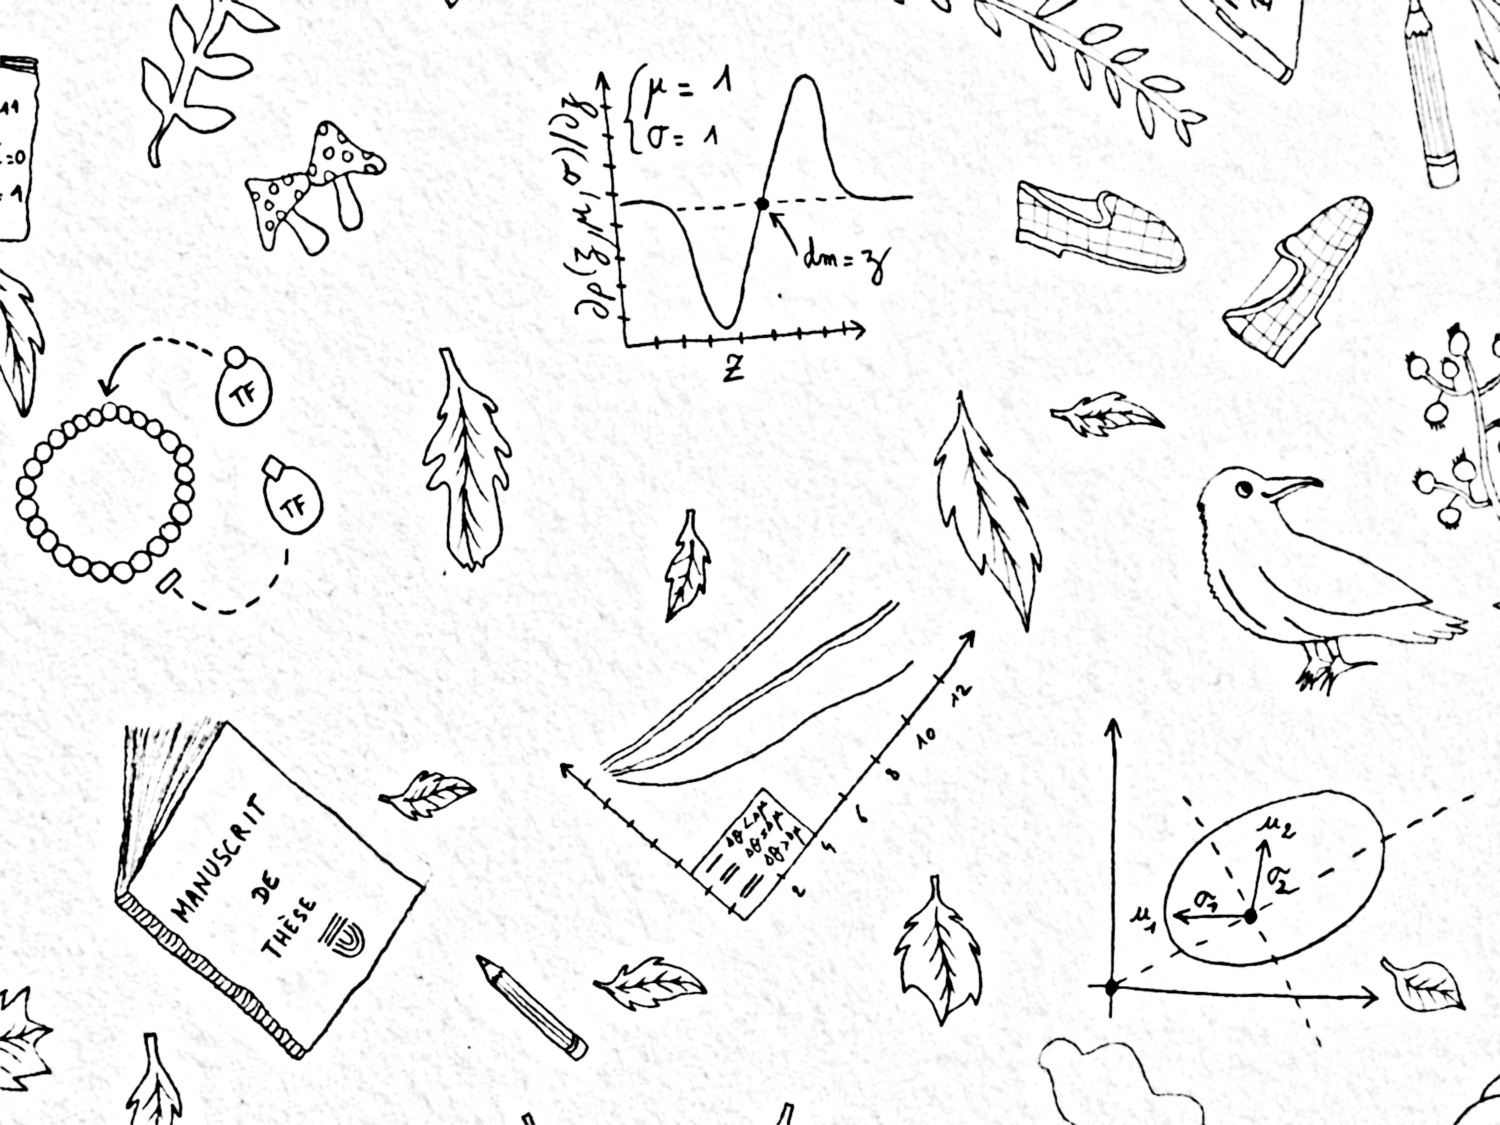
\includegraphics[width=1\textwidth]{tableau.pdf}
\caption*{\small{\textit{Par Manu\`ela, octobre 2017}}}
\end{figurehere}



